\documentclass[12pt]{article}
\usepackage{ctable,microtype,natbib,amsmath,amssymb,fullpage,graphicx}
\usepackage[colorlinks,linkcolor=black,citecolor=blue,urlcolor=black]{hyperref}
\usepackage{setspace}
%\onehalfspacing
 
\title{Anchor Finding Interface V1.0}
\author{Yoni Halpern}
 
\begin{document}
 
\maketitle{}
 

Hi! This document accompanies the initial release of the anchor interface described in: ``Using Anchors to Estimate Clinical State without Labeled Data'' by Y. Halpern, Y.D. Choi, S. Horng, D. Sontag. To appear in the American Medical Informatics Association (AMIA) Annual Symposium, Nov. 2014. 


\section{Contact Information}
Please direct questions to Yoni Halpern: halpern@cs.nyu.edu

\section{Quick Start}

\subsection{Installation}
Clone the github repository for AnchorExplorer with the following command:

\begin{verbatim}
$ git clone https://github.com/yhalpern/anchorExplorer.git
$ cd anchorExplorer
\end{verbatim}

We have tested the interface on a system with the following properties:
\begin{itemize}
\item Mac or unix OS
\item python 2.6 or 2.7
\item numpy 1.8.1 and scipy 0.13.3
\item scikit-learn 0.15
\item networkx 1.8.1
\item Tkinter Revision 81008
\item ttk 0.3.1
\end{itemize}

Required python packages are listed a file, requirements.txt and can be installed using pip:

\begin{verbatim}
$ pip install -r requirements.txt
\end{verbatim}

If you have trouble with Tkinter and ttk, try installing the ActiveState community edition of Python \url{http://www.activestate.com/activepython/}.

\subsection{Data}
To start, you need to have patient records in xml format. 
However, if you want to test that you can get things up and running with dummy data you can use the following command to generate 1000 properly formatted ``random'' patient records and store them in patients.xml.

\begin{verbatim}
$ python generate_patients.py 1000 > patients.xml
\end{verbatim}

A more realistic dataset can be created if you have access to the MIMIC-II clinical notes. Download the flat note files from \url{http://physionet.org/mimic2/flat_files/}.

\begin{verbatim}
$ python get_mimic_data.py path/to/mimic_files/00 examples/mimic_fields.txt 
> patients.xml
\end{verbatim}

This simple example only extracts data from the Notes table. More complicated data representations and structures are possible (see section~\ref{sec:custom_settings}).

\subsection{Settings}
An example settings file is provided in the examples/ directory. To customize this file for your own data, see section~\ref{sec:custom_settings}.

\subsection{Preprocess Data}

Use the preprocess\_patients.py script to preprocess the data in patients.xml for easy lookups and storage. The interface will read from the files generated by this script. Using the example settings file:

\begin{verbatim}
$ python preprocess_patients.py 1000 patients.xml examples/settings.xml
\end{verbatim}

This script does some simple negation detection, bigram detection and stopword removal.
If you wish to use your own custom language processing pipeline, see section~\ref{sec:custom_language_processing}.

\subsection{Create an anchors directory}
\begin{verbatim}
$ mkdir anchors
\end{verbatim}

\subsection{Run the interface}
To run the interface using the example settings file:

\begin{verbatim}
$ python gui.py examples/settings.xml
\end{verbatim}

\subsection{Exploring the data}
\begin{figure}[tb]
    \begin{center}
        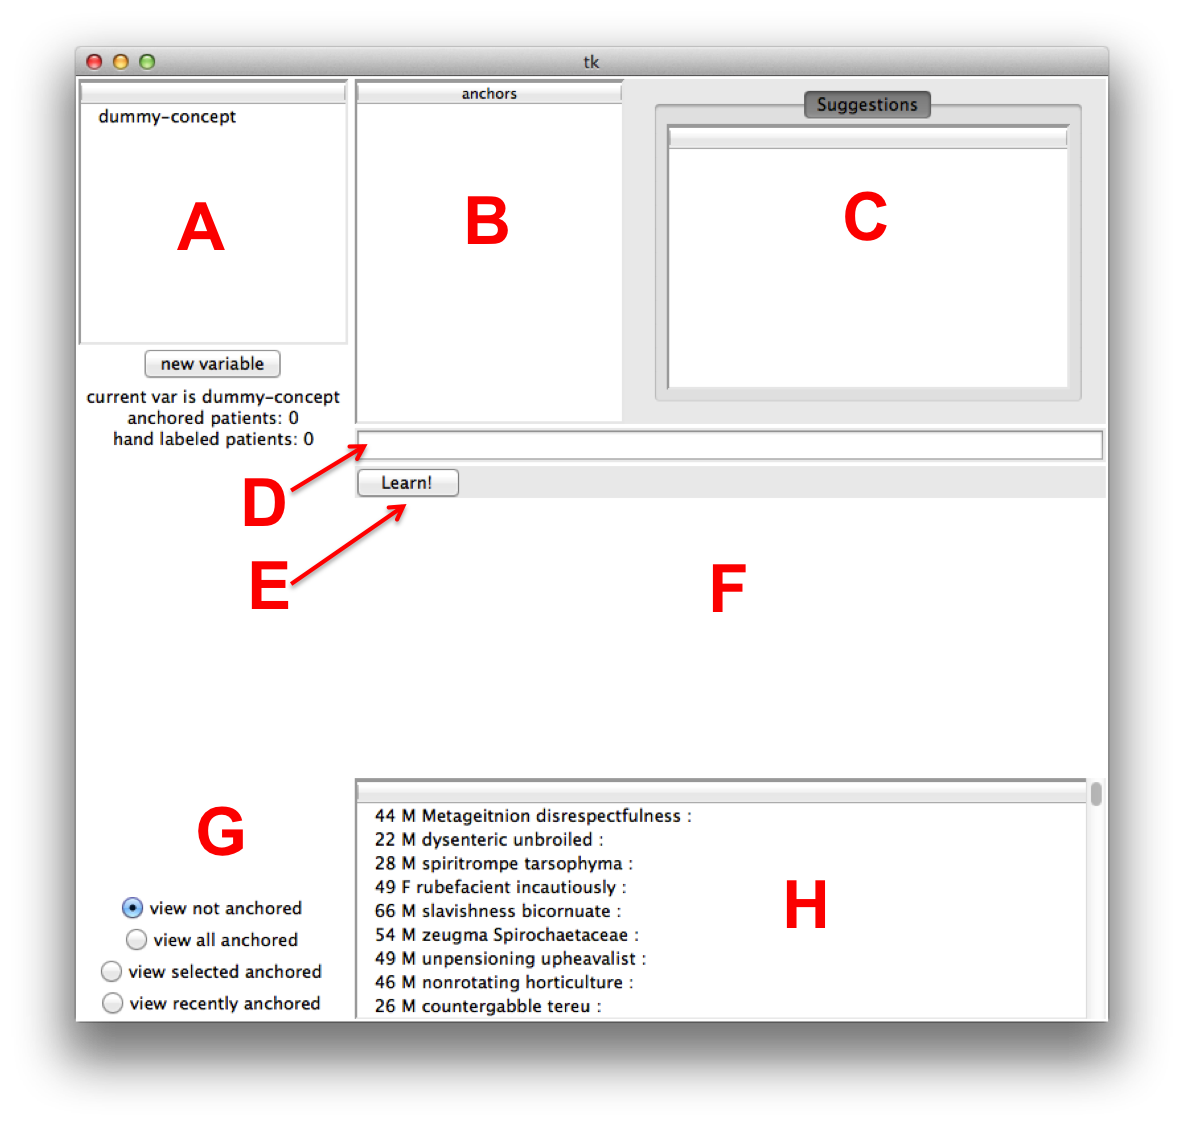
\includegraphics[scale=0.40]{screen_2_annotated.png}
        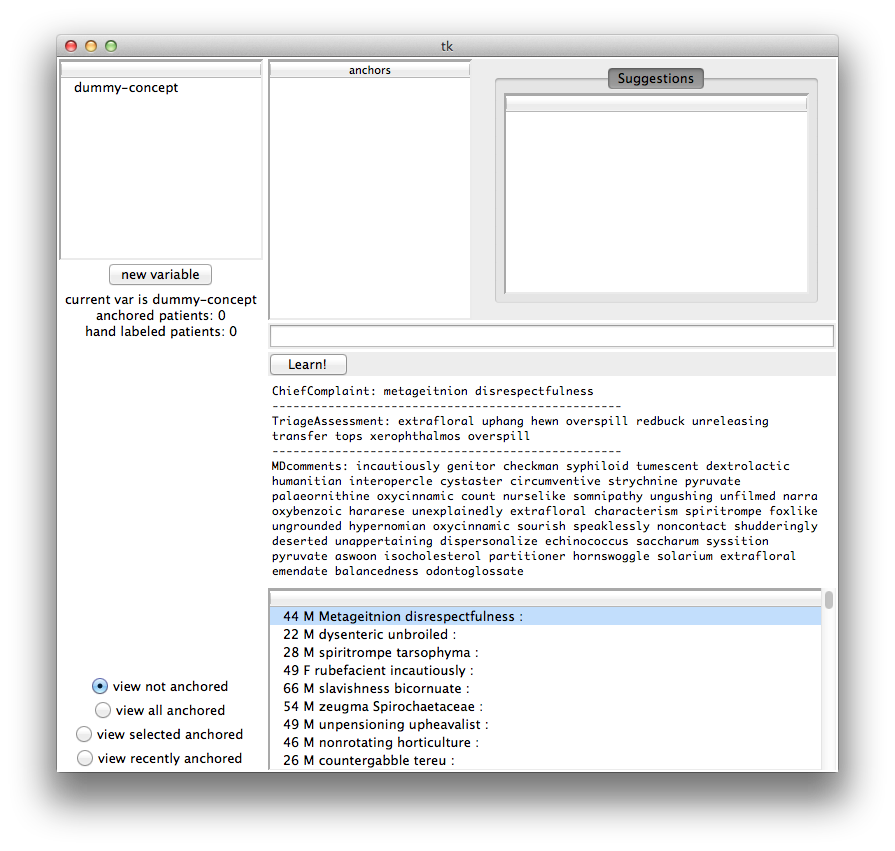
\includegraphics[scale=0.25]{screen_3.png}
    \end{center}
    \caption{\label{fig:first_activation} (Left) Screenshot when the interface is first activated. Panes are annotated in red and each one is explained in detail in Section~\ref{sec:anatomy}. (Right) Viewing a patient in more detail. Random words are inserted for patient text here.}
\end{figure}

You can explore the data on the patient visit level with the patient summary display\footnote{This display sometimes gets initialized with a height of zero at the bottom of the window and may need to be dragged up in order to be visible.} (H) and detailed display (F). Selecting a patient in the summary display shows the patient's record in more detail above it. In this simple example, we are only showing three text fields, but more data can be shown here.

\subsection{Create a new cohort}
Pushing the ``new variable'' button (below A) will pop up a dialog to create a new cohort variable. You will be prompted to provide a name.

\subsection{Adding an anchor}

Choose a word that appears in the patient data (e.g. for the randomly generated data, try ``bioluminescence'') and enter it in the text input box (D). 

\subsection{Filtering the data}

Choose to filter for patients that have the anchor or view only patients that do not have the anchor by using the radio buttons to change the filters (G).

\subsection{Learning a model}
Until now, you have just been exploring the patient data and applying filters, but no learning has taken place. Now try pushing the ``Learn'' button (E). After a few seconds, your patients should now be ranked in order of likelihood of belonging to the cohort and suggestions for additional anchors will appear in the suggestions pane (C).

\subsection{Saving state}
Try closing the window and opening it up again. Your cohorts and anchors should be preserved.

\section{Anatomy of the interface}
\label{sec:anatomy}
\subsection{Cohort Selection Menu (A)}
Allows you to select cohorts, and create new ones.
Some commands:
\begin{itemize}
\item New variable button to create a new cohort
\item `-' delete cohort
\item `r' rename cohort
\end{itemize}


\subsection{Anchor Display (B)}
Displays the current anchors for the selected topic.
Commands:
\begin{itemize}
\item Enter text into text box and push enter to add a new anchor
\item `-' delete selected anchor
\item Anchors can also be added using the anchor suggestion pane (Top Right)
\end{itemize}

\subsection{Anchor Suggestion Pane (C)}
Displays suggestions for anchors and allows for navigation and adding of structured anchors.
Commands:
\begin{itemize}
\item ``+'' to add selected anchor suggestion
%\item ``suggest'' pane gives ranked anchor suggestions.
%\item other panes give an interface to navigate structured data types (e.g. code, med, etc)
\end{itemize}
{\bf Important:} The anchor suggestions are not necessarily all good - choosing anchors requires judgment of whether to accept or reject the automated suggestions. They are  meant to trigger associations, not  tell you what makes a good anchor or not!

\subsection{Anchor Input Box (D)}
Type anchors in here, push enter to apply them. You will need to push learn to relearn the model after adding an anchor.

\subsection{Learn Button (E)}
Learns a model using the currently selected anchors.

\subsection{Detailed Patient Display (F)}
Detailed display of the patient selected in Patient List (Bottom Right). Anchors are highlighted red. Structured data types can be clicked to navigate directly to the relevant part of the hierarchy (displayed in Anchor Suggestion Pane).
\subsection{Patient Filters (G)}
Possible options here:
\begin{itemize}
\item view not anchored: patients that do not have an anchor.
\item view all anchored: all patients that have an anchor.
\item view selected anchor: view patients that have the selected anchor (selected in pane B).
\item view recent anchor: view patients added by the most recent anchor.
\end{itemize}

\subsection{Patient List (H)}
List of patients with summary information. 
These patients can be filtered using the radio buttons on the left (e.g. view all anchored, view not anchored, etc).
After the concept has been ``learned'' using the Learn Button, this list will be ranked in order of how highly the patient fits the currently selected concept.

Usage:
\begin{itemize}
\item arrow keys to navigate
\item ``+'' mark patient as a positive example
\item ``-'' mark patient as a negative example
\item ``0'' remove patient markings
\end{itemize}


\section{Customizations}
This section is still incomplete, more information coming here shortly. Please contact if you have questions about how to use this tool on your data.

\subsection{patientSets}
This section describes which patients should be selected for visualization. If you have many patients, the interface may run slowly, here you can show that you only want to use the first 10,000 patients for an initial exploration.

\begin{verbatim}
1. <patientSets>
2.    <set name='train' start='0' end='10000'/>
3.    <set name='validate' start='0' end='15000'/>
4. </patientSets>
\end{verbatim}

The only important patientSet in this version of the code are the ``train'' and ``validate'' set. 
The start and end fields indicate indices of patients as they are listed in the file visitIDs which is generated by the preprocessing script.
Only patients from the validate set are shown. Patients in the train set are not shown.

\subsection{Language Parsing}
\label{sec:custom_language_processing}
Coming soon... more information on customizing the language parser.


\subsection{Data Fields}
\label{sec:custom_settings}
Use the settings.xml file to customize the interface for your particular dataset. An example settings.xml file is provided along with the interface code in the examples directory. Most of it can be left as is. The most important parts to customize are the {\tt dataTypes} and {\tt displaySettings} sections.


\subsubsection{Data Types}
\label{sec:dataTypes}
We divide data into different {\em types} (e.g. text, age, sex, medications, diagnoses, procedures, etc.). Each type is denoted by a {\tt datum} tag and contains a number of {\tt field} tags that describe where this data appears in a patient xml representation.

For example, here is a sample patient representation in xml format generated by the random patient generator:

\begin{verbatim}
//patient.xml
<visit>
  <index>qVwLYjLKqlkZhvkf</index>
  <MDcomments> SOME TEXT</MDcomments>
  <Age> 44 </Age>
  <Sex>M</Sex>
  <ChiefComplaint> SOME TEXT</ChiefComplaint>
  <TriageAssessment>SOME TEXT</TriageAssessment>
</visit>
\end{verbatim}
{\bf Important}: Every patient instance must be enclosed in a {\tt visit} tag and must have a unique {\tt index} tag. All other fields are customizable.
Here is a section of settings.xml that could be used for patient records with this schema.

\begin{verbatim}
//settings.xml
1. <datum type=`text' heirarchy=`' prefix=`'>
2.     <field name=`MDcomments' path=`.'/>
3.     <field name=`ChiefComplaint' path=`.'/>
4.     <field name=`TriageAssessment' path=`.'/>
5. </datum>
\end{verbatim}

Line 1 of settings.xml says that there is a type of data called {\bf text}. That it is not hierarchical and that it should not be represented with any special prefix.

Lines 2-4 show where in the patient records it can be found (ie. the MDcomments, ChiefComplaint and TriageAssessment sections). The final representation of the {\bf text} data will be a concatenation of these three fields.

\subsubsection{Display Settings}
\label{sec:display_settings}
For each type of data described in Section~\ref{sec:dataTypes}, you may want to customize where it is displayed (or whether it is displayed at all). Here you can specify what appears in the {\tt patientSummary} section and the {\tt detailedDisplay}. 

The following snippet says that Age, Sex and ChiefComplaint should be displayed as the patient summary:
\begin{verbatim}
<patientSummary>
    <displayFields>
        <field name='Age'/>
        <field name='Sex'/>
        <field name='ChiefComplaint'/>
    </displayFields>
</patientSummary>
\end{verbatim}

And the following snippet says that ChiefComplaint, TriageAssessment, MDcomments should be displayed in the detailed patient description:

\begin{verbatim}
<detailedDisplay>
    <displayFields>
        <field name='ChiefComplaint' path='.'/>
        <field name='TriageAssessment' path='.'/>
        <field name='MDcomments' path='.'/>
    </displayFields>
</detailedDisplay>
\end{verbatim}

The resulting display is shown in Figure~\ref{patientDisplay}.
\begin{figure}[ht]
	\begin{center}
		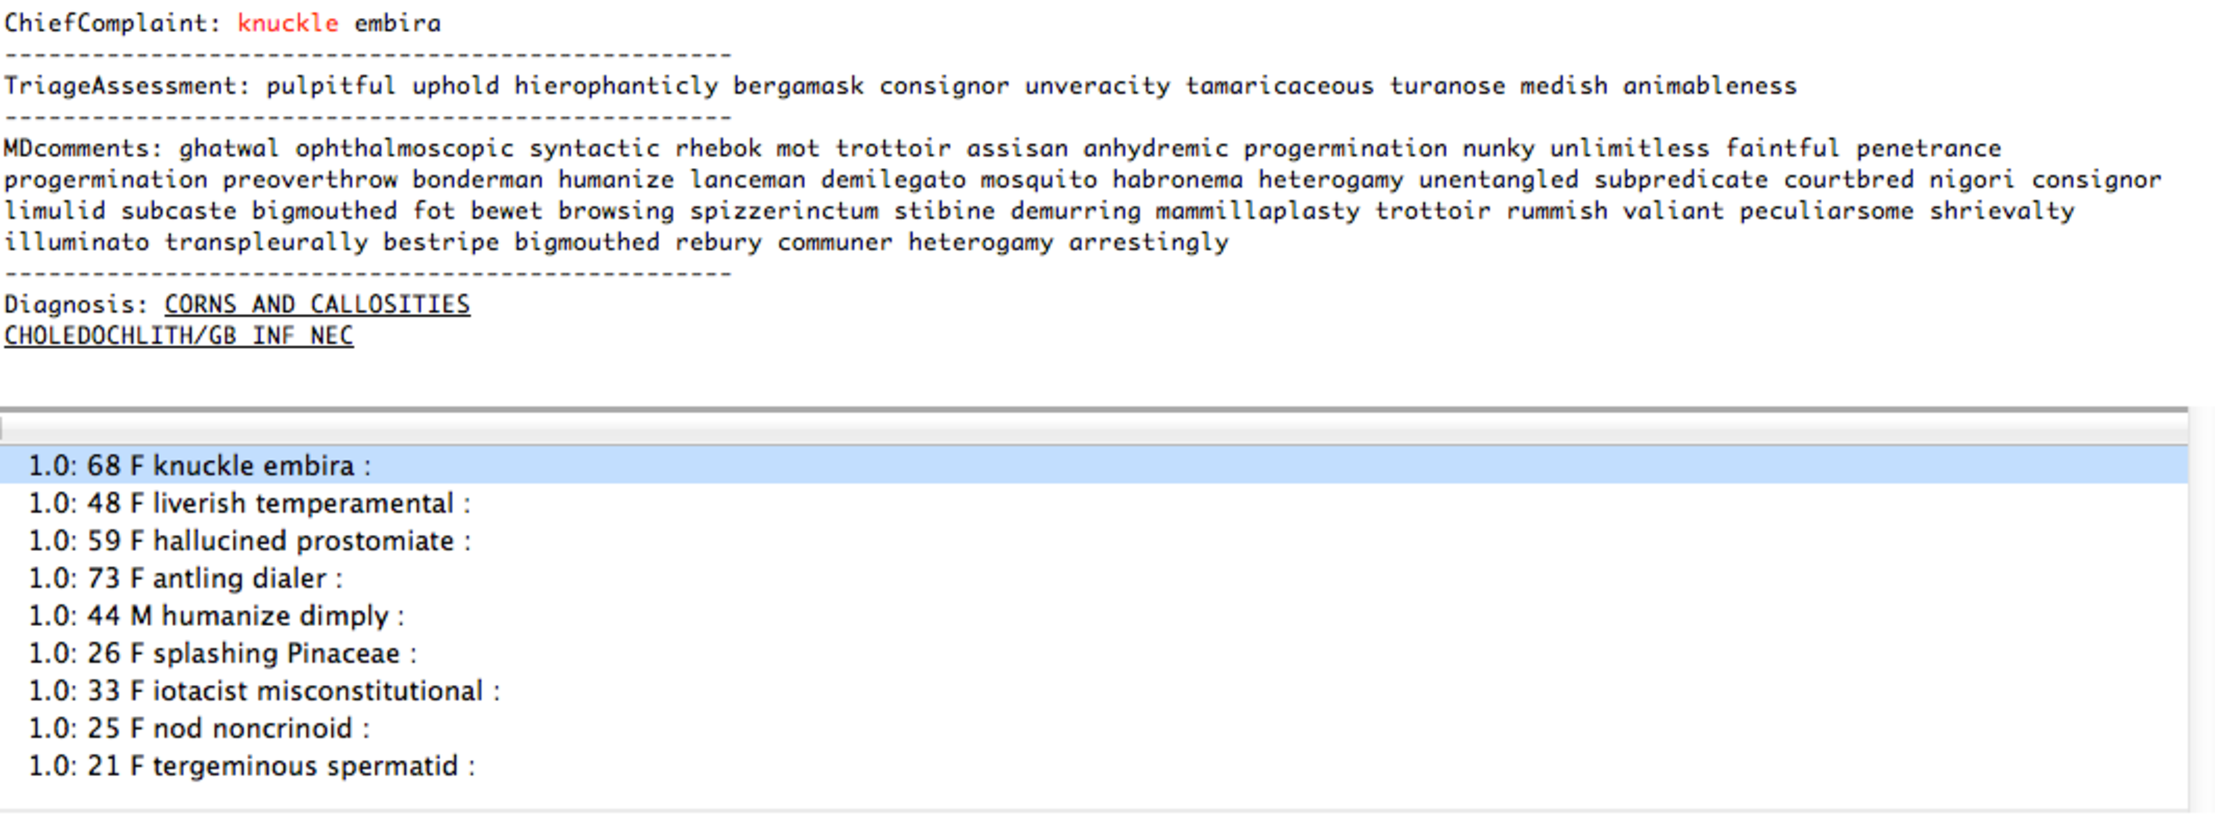
\includegraphics[scale=0.5]{patientDisplayScreenshot}
	\end{center}
	\caption{\label{patientDisplay} Customizing the patient display as described in section~\ref{sec:display_settings}. The bottom list view shows Age, Sex and Chief Complaint for every patient. The top detailed view of a single patient shows fields: ChiefComplaint, TriageAssessment,MDcomments. We display random words instead of real patient notes.}
	\label{fig:figure1}
\end{figure}

\subsection{Structured Data Types}
Some data elements can be described as belonging to a hierarchy of items, (e.g. ICD9 codes, NDC codes, etc). 
We support exploring data hierarchies and adding anchors from hierarchically typed data.
In the following section, we demo this capability in order to view diagnosis codes in MIMIC data alongside text.

\subsection{Customization demo}
\label{sec:customization demo}
This demo will walk you through how to include a new data field, in this case ICD9 codes to be viewed in the user interface. It assumes that you have access to MIMIC-II data.

(The commands from this demo can be found in a script run\_mimic.sh which takes a single argument which is the path to the mimic-II flat files). 

As before, we begin by formatting the patient data in a patients.xml file.
\begin{verbatim}
$ python get_mimic_data.py path/to/mimic_files/00 examples/mimic_fields.txt 
> patients.xml
\end{verbatim}

Looking at the patients.xml file, you will see that ICD9 codes are recorded in the dataset.

We would like to create a {\em data dictionary} to map these codes to plaintext and a {\em data structure} to store these codes in a hierarchical manner.

First we need two tab-separated files that will store this data: X.names and X.edges. 
In general we assume that the user supplies these files for any structured data type of interest.
For this example, we provide a script examples/ICD9/load\_ICD9\_structure.py which downloads the ICD9 hierarchy from a public git repository and creates these formatted files. {\bf This hierarchy is incomplete and does not contain entries for every ICD9 code in MIMIC-II, but it serves as a good illustration}.

\begin{verbatim}
$ cd examples/ICD9
$ python load_ICD9_structure.py
\end{verbatim}

We now want to build these into the structured format that the interface reads from.
\begin{verbatim}
$ cd ../..
$ python build_structured_rep.py code examples/ICD9/code
$ ls Structures
codeDict.pk    codeStruct.pk
\end{verbatim}

Now we need to update settings.xml to recognize this new structured data type. An example settings file is found in examples/ICD9/settings.xml. Below is an excerpt of the relevant lines:

\begin{verbatim}
#lines 28-30
 <datum type='code' heirarchy='Structures/codeStruct.pk' prefix='code_'
  dictionary='Structures/codeDict.pk' realtime='true'>
    <field name='Diagnosis' path='D_code' display='D_name'/>
 </datum>
 \end{verbatim}

 \begin{verbatim}
 #lines 41-45
 <displayFields>
    <field name='ChiefComplaint' path='.'/>
    <field name='TriageAssessment' path='.'/>
    <field name='MDcomments' path='.'/>
    <field name='Diagnosis' path='.'/>
 </displayFields>
\end{verbatim}

We can now run the preprocessing script to import the data with the structured ICD9 codes included.

\begin{verbatim}
$ python preprocess_patients.py 1000 patients.xml examples/ICD9/settings.xml
\end{verbatim}

And run the interface:
\begin{verbatim}
$ python gui.py examples/ICD9/settings.xml
\end{verbatim}

Now next to the suggestions pane there should be an option `code' which will display ICD9 codes in a structured version that can be added to the anchor list with the `+' key. Adding a parent in the hierarchy will add all of the children.

\section{More Information}
Contact: Yoni Halpern - halpern@cs.nyu.edu
\end{document}
